\documentclass[11pt]{article}

\usepackage[a4paper,margin=1in]{geometry}
\usepackage{graphicx}
\usepackage{float}
\usepackage{booktabs}
\usepackage{amsmath}
\usepackage{titlesec}
\usepackage{setspace}
\usepackage{caption}

\setstretch{1.08}
\captionsetup{font=small}

\title{\textbf{Impact of Link Error Rate on MANET Routing Performance in ns-3}}
\author{}
\date{}

\begin{document}

\maketitle

\section{Introduction}

This report presents a comparative ns-3 based performance analysis of four MANET routing protocols under increasing channel error rates: AODV, AOMDV, DSDV, and OLSR. In this experiment, the network configuration was kept fixed and only the error rate was varied. The goal was to study how protocol behavior changes as link reliability degrades, and to understand whether multipath routing in AOMDV provides measurable improvement over the single-path AODV protocol.

The main performance metrics considered are Packet Delivery Ratio (PDR), throughput, average delay, routing overhead, and packet loss rate.

\section{Network Topologies Under Simulation}

The simulations were conducted on a wireless MANET topology. All protocols were evaluated under the same underlying network setup so that the effect of error rate could be isolated fairly.

The common simulation setting was:

\begin{itemize}
    \item Wireless mobile ad hoc network (MANET)
    \item Number of nodes: 10
    \item Number of flows: 10
    \item Node speed: 20 m/s
    \item Pause time: fixed
    \item Simulation time: 20 s
    \item Packet size: 512 bytes
\end{itemize}

The routing protocols compared were:

\begin{itemize}
    \item AODV
    \item AOMDV (implemented from scratch)
    \item DSDV
    \item OLSR
\end{itemize}

\section{Parameter Under Variation}

In this study, only the \textbf{link error rate} was varied, while all other simulation parameters were kept constant.

The tested error-rate conditions were:

\begin{itemize}
    \item 0\% error
    \item 10\% error
    \item 20\% error
\end{itemize}

This setup makes the comparison more meaningful, since any observed change in performance can be attributed directly to increasing channel unreliability rather than to changes in topology size, flow count, or mobility.

\section{Results with Graphs}

\subsection{Protocol Comparison Across Error Rates}

\begin{figure}[H]
    \centering
    
\includegraphics[width=\textwidth]{protocol_comparison.png}
    \caption{Comparison of AODV, DSDV, and OLSR under 0\%, 10\%, and 20\% error rates.}
\end{figure}

Figure 1 shows that increasing error rate degrades all protocols, but the extent of degradation differs significantly. AODV achieves the best PDR and throughput under zero error, but its delay grows very sharply once errors are introduced. DSDV shows moderate throughput and delivery performance, but its packet loss remains relatively high across all cases. OLSR maintains comparatively low packet loss and good robustness under higher error, though its throughput stays lower than AODV at baseline.

\begin{table}[H]
    \centering
    \small
    \caption{0\% error: AODV, DSDV, OLSR metrics}
    \begin{tabular}{lccccc}
        \toprule
        Protocol & PDR (\%) & Throughput (kbps) & Delay (ms) & Loss (\%) & Routing OH \\
        \midrule
        AODV & 92.31 & 241.27 & 86.18 & 2.89 & 0.1678 \\
        DSDV & 65.12 & 170.21 & 418.63 & 15.70 & 0.0000 \\
        OLSR & 84.12 & 196.78 & 52.60 & 1.11 & 0.0000 \\
        \bottomrule
    \end{tabular}
\end{table}

\begin{table}[H]
    \centering
    \small
    \caption{10\% error: AODV, DSDV, OLSR metrics}
    \begin{tabular}{lccccc}
        \toprule
        Protocol & PDR (\%) & Throughput (kbps) & Delay (ms) & Loss (\%) & Routing OH \\
        \midrule
        AODV & 75.62 & 197.64 & 765.52 & 16.45 & 0.2331 \\
        DSDV & 50.74 & 132.62 & 461.83 & 18.51 & 0.0000 \\
        OLSR & 79.14 & 123.77 & 173.33 & 8.15 & 0.0000 \\
        \bottomrule
    \end{tabular}
\end{table}

\begin{table}[H]
    \centering
    \small
    \caption{20\% error: AODV, DSDV, OLSR metrics}
    \begin{tabular}{lccccc}
        \toprule
        Protocol & PDR (\%) & Throughput (kbps) & Delay (ms) & Loss (\%) & Routing OH \\
        \midrule
        AODV & 59.09 & 154.44 & 812.25 & 24.71 & 0.0661 \\
        DSDV & 44.79 & 117.07 & 500.41 & 20.50 & 0.0000 \\
        OLSR & 77.93 & 119.02 & 205.49 & 9.76 & 0.0000 \\
        \bottomrule
    \end{tabular}
\end{table}

\subsection{AODV vs AOMDV Under Error Variation}

\begin{figure}[H]
    \centering
    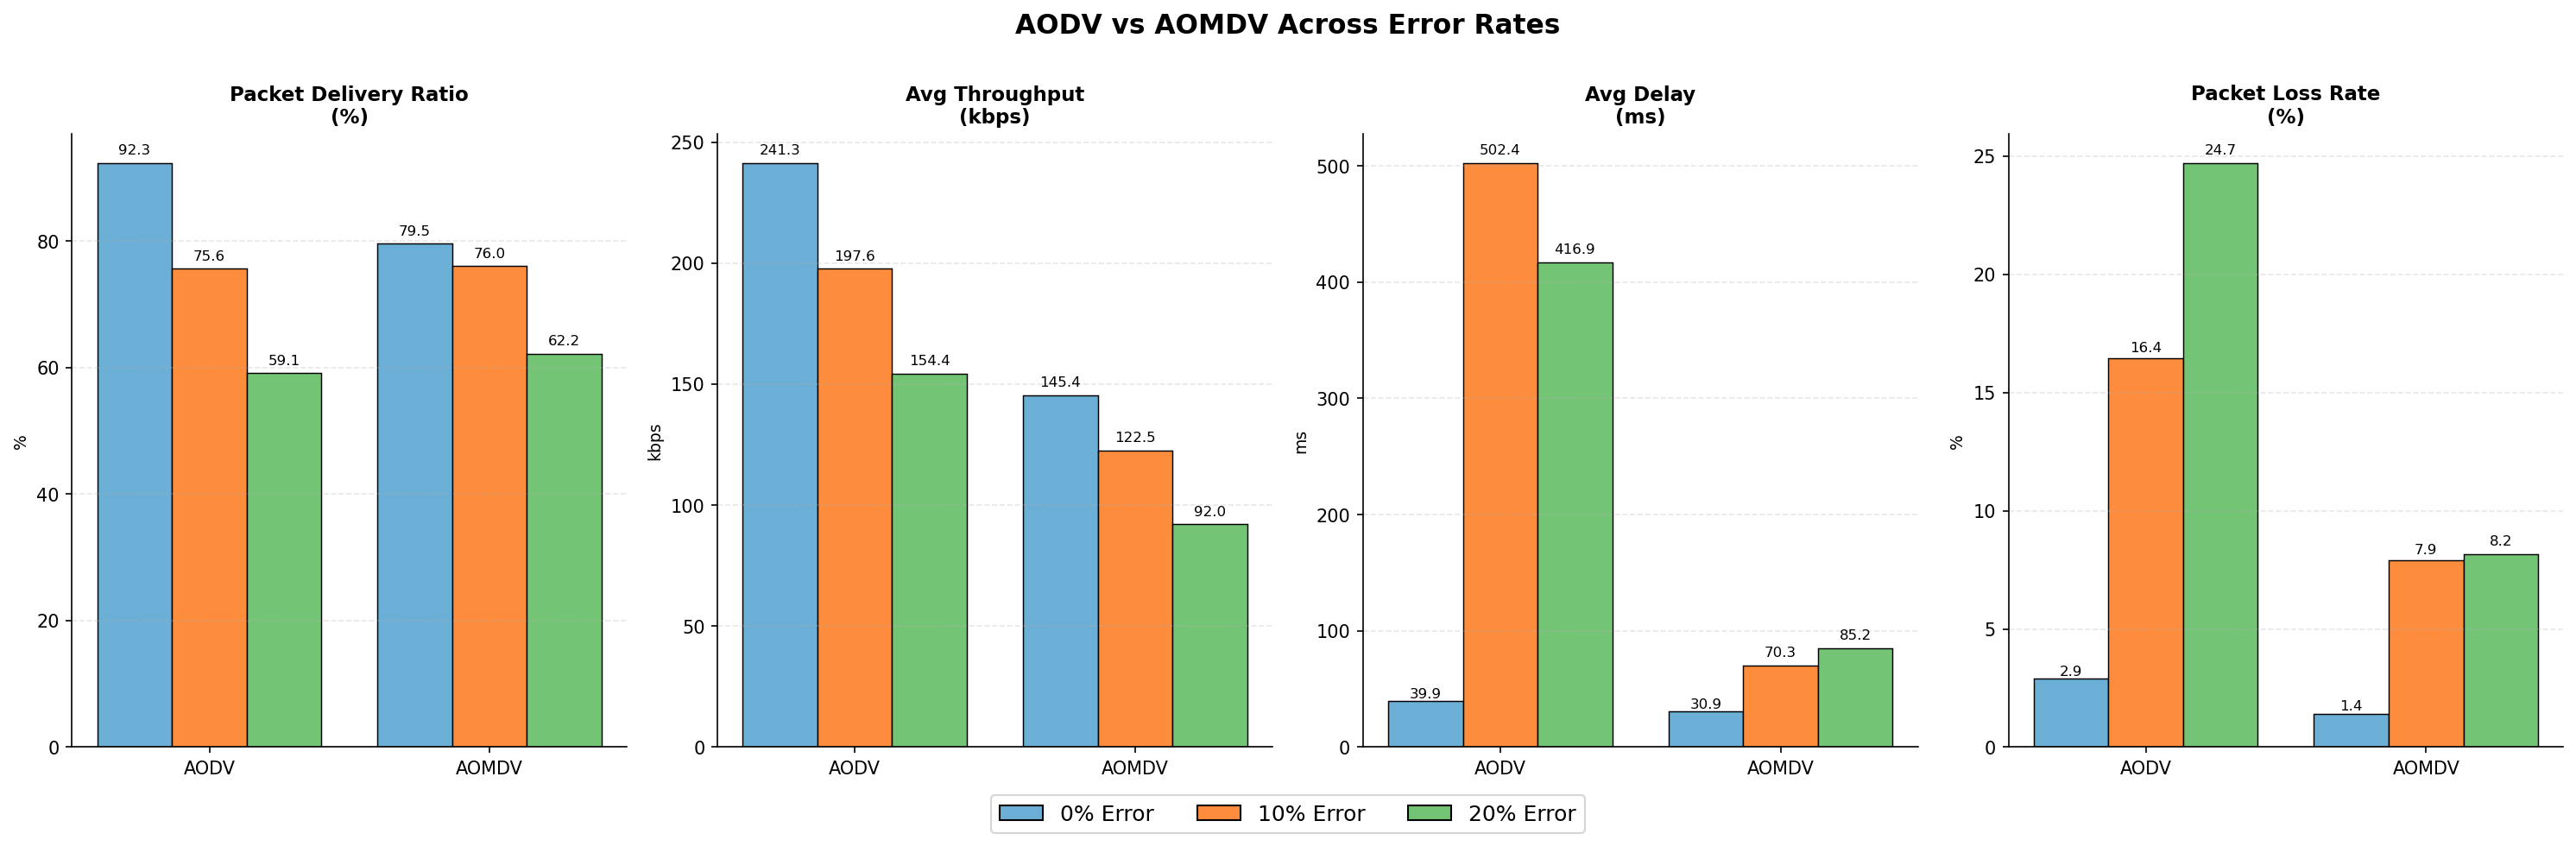
\includegraphics[width=\textwidth]{aodv_aomdv_comparison.png}
    \caption{Direct comparison between AODV and AOMDV across increasing error rates.}
\end{figure}

Figure 2 highlights the specific impact of multipath routing. At 0\% error, AODV slightly outperforms AOMDV in PDR and throughput. However, as the error rate increases to 10\% and 20\%, AOMDV clearly becomes more resilient. It delivers lower delay and lower packet loss than AODV under both impaired conditions, showing the benefit of maintaining alternate paths when the primary path becomes unreliable.

\begin{table}[H]
    \centering
    \small
    \caption{AODV vs AOMDV: delivery and throughput across error rates}
    \begin{tabular}{ccccc}
        \toprule
        Error (\%) & AODV PDR (\%) & AOMDV PDR (\%) & AODV Thpt (kbps) & AOMDV Thpt (kbps) \\
        \midrule
        0 & 92.31 & 79.55 & 241.30 & 145.40 \\
        10 & 75.62 & 76.01 & 197.60 & 122.50 \\
        20 & 59.09 & 62.19 & 154.40 & 92.02 \\
        \bottomrule
    \end{tabular}
\end{table}

\begin{table}[H]
    \centering
    \small
    \caption{AODV vs AOMDV: delay and packet loss across error rates}
    \begin{tabular}{ccccc}
        \toprule
        Error (\%) & AODV Delay (ms) & AOMDV Delay (ms) & AODV Loss (\%) & AOMDV Loss (\%) \\
        \midrule
        0 & 39.90 & 30.93 & 2.89 & 1.42 \\
        10 & 502.40 & 70.32 & 16.45 & 7.91 \\
        20 & 416.90 & 85.23 & 24.71 & 8.18 \\
        \bottomrule
    \end{tabular}
\end{table}

\section{Summary Findings}

The main findings of the experiment are summarized below:

\begin{itemize}
    \item Increasing error rate reduces PDR and throughput for all protocols.
    \item Average delay increases significantly as link errors grow, especially for reactive single-path routing.
    \item AODV performs best at 0\% error in terms of PDR and throughput, but degrades sharply under 10\% and 20\% error.
    \item AOMDV provides a clear improvement over AODV in lossy conditions by reducing delay and packet loss.
    \item OLSR shows stronger stability than AODV and DSDV at higher error rates, particularly in packet loss behavior.
    \item DSDV is generally weaker in delivery efficiency and throughput compared with the other protocols in this setup.
\end{itemize}

\section{Discussion and Reflection}

This experiment shows that routing behavior in MANETs depends not only on network structure and mobility, but also very strongly on channel reliability. Since all simulation settings were fixed except error rate, the observed performance trends directly reflect how each routing strategy responds to increasing link impairment.

AODV performs very well when the channel is clean. At 0\% error, it achieves the highest PDR and highest throughput among the compared protocols. This is expected because AODV is an on-demand protocol that avoids the continuous control overhead of proactive routing, so when links are stable, it can forward data efficiently using discovered routes. However, the weakness of AODV becomes obvious once errors are introduced. At 10\% and 20\% error, its average delay becomes extremely high and its packet loss rises sharply. The reason is that AODV relies on a single active route. When that route breaks or becomes unreliable, route rediscovery is needed, which increases latency and causes more dropped packets before a new path is established.

AOMDV improves on this exact limitation. Although it is derived from AODV, it maintains multiple loop-free alternative paths instead of one primary path only. That design introduces some extra control complexity, and this is why at 0\% error AOMDV does not surpass AODV in raw throughput or PDR. In a clean channel, the extra path maintenance is not fully beneficial. But once the environment becomes error-prone, the advantage becomes very clear. At both 10\% and 20\% error, AOMDV achieves much lower delay than AODV and also substantially lower packet loss. This happens because when one path becomes unreliable, the protocol can switch to a backup route instead of immediately starting a new discovery process. In practical terms, AOMDV trades a small amount of efficiency in ideal conditions for much stronger robustness in impaired conditions.

DSDV behaves differently because it is proactive and table-driven. It continuously maintains routing information, which can help reduce route acquisition delay in some cases. However, in this experiment it does not translate into strong overall performance. Its throughput is lower than AODV at baseline and lower than OLSR in several stressed cases, while packet loss remains relatively high. This suggests that the periodic table maintenance of DSDV is not enough to compensate for the cost of stale or less adaptive route information under rapidly degrading link conditions. In other words, it maintains routes continuously, but those routes are not necessarily the most resilient when error rates are high.

OLSR is also proactive, but it performs better than DSDV in this experiment. Its strongest result is its relative stability under impaired conditions. OLSR maintains the lowest packet loss among the three protocols compared in the general MANET plot and preserves comparatively good PDR at 10\% and 20\% error. This can be explained by its efficient link-state style operation and the use of optimized relay selection, which helps distribute routing knowledge more effectively. Its baseline throughput is lower than AODV, so it is not the fastest protocol in favorable conditions, but it appears more balanced when the channel becomes unreliable.

Taken together, the results suggest the following interpretation. If the environment is clean and the goal is maximum throughput with low routing complexity, AODV is attractive. If the environment is lossy or unstable, AOMDV is a better choice because it preserves communication quality more effectively by using alternate paths. OLSR offers a stable and dependable proactive alternative, especially when robustness is more important than peak throughput. DSDV, in this simulation setting, is the least competitive overall because it does not match AODV's baseline efficiency or OLSR's higher-error robustness.

The most important takeaway from this the AODV versus AOMDV comparison is that multipath routing is not mainly about improving best-case performance. Its real value appears when the network becomes unreliable. AOMDV does not need to beat AODV in ideal conditions to be useful. Its strength lies in graceful degradation. As errors increase, it loses less performance, which makes it more suitable for adverse MANET environments.

\section{Conclusion}

This report evaluated the effect of increasing error rate on MANET routing performance using ns-3. With all other parameters fixed, the results show that channel impairment has a strong negative impact on delivery ratio, throughput, delay, and packet loss. Among the compared protocols, AODV performs best in the zero-error case, but AOMDV clearly improves robustness once errors are introduced. OLSR also demonstrates stable behavior under higher error, while DSDV performs less favorably in this setup.

Overall, the study confirms that protocol choice should depend on the expected channel condition. For cleaner links, AODV remains efficient. For more unreliable networks, AOMDV provides a more fault-tolerant solution through multipath routing.

\end{document}